
\documentclass[11pt]{isuthesis}
\usepackage[]{graphicx}\usepackage[]{color}
%% maxwidth is the original width if it is less than linewidth
%% otherwise use linewidth (to make sure the graphics do not exceed the margin)
\makeatletter
\def\maxwidth{ %
  \ifdim\Gin@nat@width>\linewidth
    \linewidth
  \else
    \Gin@nat@width
  \fi
}
\makeatother

\definecolor{fgcolor}{rgb}{0.345, 0.345, 0.345}
\newcommand{\hlnum}[1]{\textcolor[rgb]{0.686,0.059,0.569}{#1}}%
\newcommand{\hlstr}[1]{\textcolor[rgb]{0.192,0.494,0.8}{#1}}%
\newcommand{\hlcom}[1]{\textcolor[rgb]{0.678,0.584,0.686}{\textit{#1}}}%
\newcommand{\hlopt}[1]{\textcolor[rgb]{0,0,0}{#1}}%
\newcommand{\hlstd}[1]{\textcolor[rgb]{0.345,0.345,0.345}{#1}}%
\newcommand{\hlkwa}[1]{\textcolor[rgb]{0.161,0.373,0.58}{\textbf{#1}}}%
\newcommand{\hlkwb}[1]{\textcolor[rgb]{0.69,0.353,0.396}{#1}}%
\newcommand{\hlkwc}[1]{\textcolor[rgb]{0.333,0.667,0.333}{#1}}%
\newcommand{\hlkwd}[1]{\textcolor[rgb]{0.737,0.353,0.396}{\textbf{#1}}}%

\usepackage{framed}
\makeatletter
\newenvironment{kframe}{%
 \def\at@end@of@kframe{}%
 \ifinner\ifhmode%
  \def\at@end@of@kframe{\end{minipage}}%
  \begin{minipage}{\columnwidth}%
 \fi\fi%
 \def\FrameCommand##1{\hskip\@totalleftmargin \hskip-\fboxsep
 \colorbox{shadecolor}{##1}\hskip-\fboxsep
     % There is no \\@totalrightmargin, so:
     \hskip-\linewidth \hskip-\@totalleftmargin \hskip\columnwidth}%
 \MakeFramed {\advance\hsize-\width
   \@totalleftmargin\z@ \linewidth\hsize
   \@setminipage}}%
 {\par\unskip\endMakeFramed%
 \at@end@of@kframe}
\makeatother

\definecolor{shadecolor}{rgb}{.97, .97, .97}
\definecolor{messagecolor}{rgb}{0, 0, 0}
\definecolor{warningcolor}{rgb}{1, 0, 1}
\definecolor{errorcolor}{rgb}{1, 0, 0}
\newenvironment{knitrout}{}{} % an empty environment to be redefined in TeX

\usepackage{alltt}
\newcommand{\SweaveOpts}[1]{}  % do not interfere with LaTeX
\newcommand{\SweaveInput}[1]{} % because they are not real TeX commands
\newcommand{\Sexpr}[1]{}       % will only be parsed by R


%---------------------------------------------------
\usepackage{color}
\usepackage[dvipsnames,svgnames]{xcolor}
\usepackage{wrapfig,float}
\usepackage{caption}
\usepackage{subcaption}
\usepackage{graphicx}
\usepackage{amssymb}
\usepackage{amsmath}
\usepackage{url}
\usepackage{ulem}
\usepackage[section]{placeins}
\usepackage{sidecap}
\usepackage{multirow}
\usepackage{bbm}
\usepackage[colorinlistoftodos]{todonotes}
%---------------------------------------------------

% Standard, old-style thesis
\usepackage{isutraditional}   \chaptertitle
% Old-style, thesis numbering down to subsubsection
\alternate
\usepackage{rotating}
% Bibliography without numbers or labels
\usepackage{natbib}
\bibliographystyle{apa}
%\includeonly{titletoc,chapter1}
%Optional Package to add PDF bookmarks and hypertext links
\usepackage[pdftex,hypertexnames=false,linktocpage=true]{hyperref}
\hypersetup{colorlinks=true,linkcolor=blue,anchorcolor=blue,citecolor=blue,filecolor=blue,urlcolor=blue,bookmarksnumbered=true,pdfview=FitB}

\newcommand{\done}[2][inline]{\todo[color=SpringGreen, #1]{#2}}  % for todos that have been seen and dealt with
\newcommand{\meh}[2][inline]{\todo[color=White, #1]{#2}}   % for todos that may no longer be relevant 
\newcommand{\comment}[2][inline]{\todo[color=SkyBlue, #1]{#2}} % for comments that may not be "to-do"s
\newcommand{\mcomment}[1]{\todo[color=SkyBlue]{#1}} % for margin comments

\newcommand{\newtext}[1]{\todo[inline, color=White]{ \color{OliveGreen}{#1}}} % new text - not necessarily something to be done

\newcommand{\move}[1]{\todo[inline, color=Lime]{#1}} % new to do item

%---------------------------------------------------




\begin{document}

\graphicspath{{Figure/LitReview/}{Images/LitReview/}}
\renewcommand{\floatpagefraction}{.99}





% Chapter 1 of the Thesis Template File
\chapter{OVERVIEW}

\section{Goals of Statistical Graphics}

\section{The Human Visual System}
Basic overview of structure, to serve as a reference

In order to design graphics for the human perceptual system, we must understand, at a basic level, the makeup of the perceptual system. There are multiple levels of perception that must correctly function in order to perceive visual stimuli successfully, but a somewhat simplistic higher-level analogy would be that we must understand both the hardware and software of the human visual system to create effective graphics.
The ``hardware", in this analogy, consists of the neurons that make up the eyes, optic nerve, and the brain itself. The higher-level functions (object recognition, working memory, etc.) comprise the ``software" component. In addition, much like computer software, there are different programs running simultaneously; these programs may interact with each other, run sequentially, or run in parallel. The following sections provide an overview of the grey-matter (hardware) components of the visual system as well as the higher-level cognitive heuristics (software) that order the raw input and construct our visual environment. 

\subsection{Hardware}
The physiology of perception is complex; what follows is a high-level overview of the physiology of perception, focusing on the areas most important to the perception of statistical graphics. This physiological information is important in understanding the difference between the sensation (i.e. the retinal image) and the perception (the corresponding mental representation), which is an important distinction in understanding how statistical graphics are perceived. 

\paragraph{The Eye}
The eye is a complex apparatus, but for our purposes, the primary component of the eye is the retina, which contains the sensory cells responsible for transforming light waves into electrical information in the form of neural signals. 
These sensory cells are specialized neurons, known as rods and cones, which perceive light intensity (brightness) and wavelength (color), respectively. One section of the retina, known as the fovea, contains only cones; the rest of the retina contains a mixture of rods and cones. Figure \ref{fig:retina} depicts the structure of the eye with a closeup of the retina. 

\begin{figure}
\centering
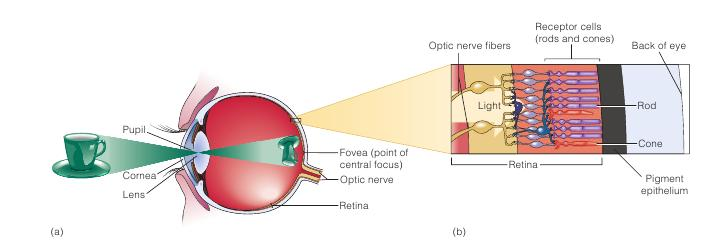
\includegraphics[width=.8\textwidth, keepaspectratio=TRUE]{Figure/LitReview/Retina}
\caption[The human eye, with closeup of receptor cells in the retina]{The human eye, with closeup of receptor cells in the retina (image from \protect\citealt{goldstein}, chap 3.1).} \label{fig:retina}
\end{figure}

\begin{figure}
\centering
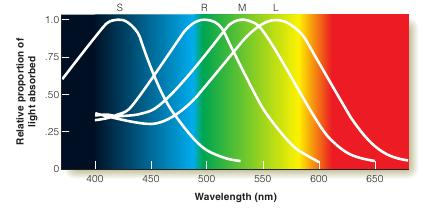
\includegraphics[width=.8\textwidth, keepaspectratio=TRUE]{Figure/LitReview/AbsorptionSpectra}
\caption[Absorption spectra of retinal cells]{Absorption spectra of rods and short, medium, and long wave cones. (image from \protect\citealt{goldstein}, chap 3.3).} \label{fig:ColorRange}
\end{figure}

Figure \ref{fig:ColorRange} shows the responsiveness of rods and each of the three types of cones to wavelengths of light in the visual spectrum. This image suggests that we have relatively good visual discrimination of the yellow-green portion of the color spectrum, but relatively poor discrimination of colors in the red and blue portions of the color spectrum. As a result, rainbow-style color schemes are seldom appropriate for conveying numerical values, because the correspondance between the perceived information and the displayed information is not accurately maintained by the visual system \citep{rainbowcolor}. In addition, if any of the cones are missing or damaged as a result of genetic mutations, color perception is impaired, resulting in a smaller range of distinguishable colors. This set of impairments is known coloquially as color-blindness, and occurs in an estimated 5\% of the population. 

\paragraph{The Brain}
Once light hits the retina and causes a signal in the receptor cells, the information travels along the optic nerve and into the brain. Multiple neighboring rods are connected to the same neuron, where each cone is connected to its' own neuron. The combined wiring of rod cells is responsible for the Hermann grid illusion and the Mach bands seen in Figure \ref{fig:InhibitionIllusions}. Both of these illusions are a product of lateral inhibition, which is a result of the wiring of rod cells in the retina.  The specifics of the wiring of the receptor cells are somewhat complex; a more thorough explanation can be found in \citet{goldstein}, chapter 3.4. 

\begin{figure}
\centering
\begin{subfigure}[b]{.45\textwidth}
  \centering
  
\includegraphics[width=\textwidth]{Figure/LitReview/HermannGrid}
  \caption{\small Hermann Grid Illusion \label{fig:hermanngrid}}
\end{subfigure}\hfill
\begin{subfigure}[b]{.45\textwidth}
  \centering
  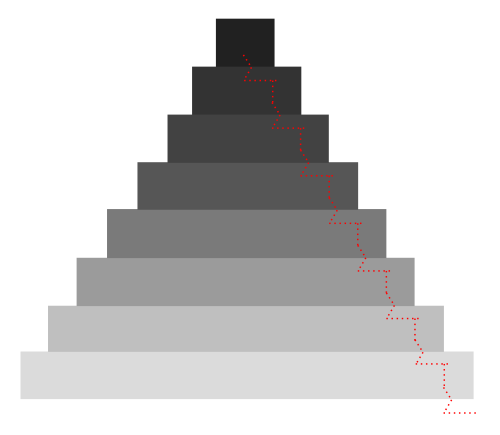
\includegraphics[width=\textwidth]{Figure/LitReview/MachBands}
  \caption{\small Mach Bands. 
  \label{fig:machbands}}
\end{subfigure}
\caption[Inhibition Illusions]{Optical Illusions resulting from lateral inhibition. The Hermann Grid illusion causes dark circles to appear at the intersection of white lines; the Mach bands illusion causes the borders of adjacent rectangles to appear more strongly defined.} \label{fig:InhibitionIllusions}
\end{figure}

Once neural impulses have left the retina through the optic nerve, they travel to the visual cortex by way of several specialized structures within the brain that process lower-level signals. Receptor cells in the visual cortext respond to specific angles, spatial locations, colors, and intensities, and arrays of these special 'feature detector cells' process the information into a form that higher-level processes can utilize. These higher-level processes are what we have previously called 'software': they are not directly related to the physical brain, but they do process information heuristically to produce higher-level reasoning and conclusions. In the next section, we explore some of the higher-level processes responsible for visual perception.

\subsection{Software}
Many of the processes for visual perception run simultaneously; in absence of a temporal ordering, we will start with the more basic tasks of visual perception and proceed towards higher-level processes. We will begin with attention.

\subsubsection{Attention and Perception} \label{AttentionPerception}
In many tasks, it is necessary to pay attention to many different input streams simultaneously; this is particularly true for complex tasks like driving a car. These tasks demand divided attention; the brain must process many different sources of information in parallel. By contrast, most image recognition tasks require selective attention, that is, focusing on specific objects and ignoring everything else. The brain accomplishes this attention through several mechanisms. 

Selective attention is accomplished by focusing the fovea (the area with the highest visual acuity) on the object. For instance, if the object is a page of text, each word will pass through the fovea, producing a focused stream of visual input. This stream of input consists of saccades (jumps between points of focus) and pauses in which the visual information is relayed to the brain. Figure \ref{fig:saccadestext} shows the saccades (lines) and pauses (circles) resulting when someone scans a paragraph of text. These saccades and pauses are utilized in eye-tracking technology to determine which parts of an image the observer is focusing on (and by extension, which information is being encoded by the brain). 

\begin{figure}[h]
\centering
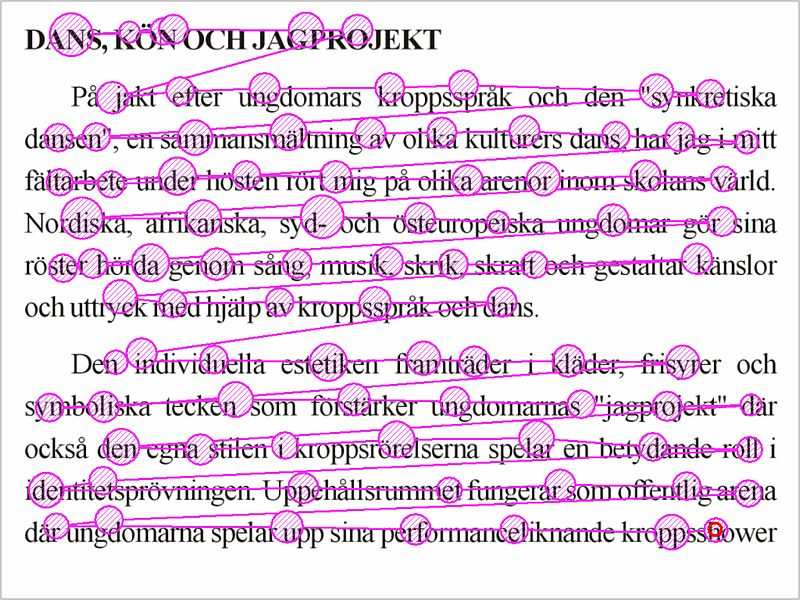
\includegraphics[width=.5\textwidth]{SaccadesText}
\caption[Saccades and Pauses]{A plot of saccades made while reading text. Saccades, shown by the lines, indicate ``jumps", while pauses are shown by circles, with size proportional to the time spent focusing on that area.}\label{fig:saccadestext}
\end{figure}

Selective attention is generally necessary for perception to occur, though there is some information that is encoded automatically. Experiments such as the fairly famous \href{http://www.theinvisiblegorilla.com/videos.html}{"gorilla" film}\footnote{\url{http://www.theinvisiblegorilla.com/videos.html}} demonstrate that even when there is attention focused on a task, information extraneous to that task is not always encoded, that is, even when participants focused on counting the number of passes of the basketball, they did not notice the obvious gorilla walking through the scene. It is important to understand which parts of a visual stimulus are the focus of a given perceptual task, because most of the information encoded by the brain is a result of selective attention. Eye-tracking can be an important tool useful to understand these perceptual processes, but participants are often able to report which parts of a stimulus contributed to their decision as well.

Within the brain, attention is important because it allows different regions of the brain which process color, shape, and position to integrate these perceptions into a multifaceted mental representation of the object \citep{goldstein}. This process, known as binding, is essential to coherently encode a scene into working memory. Feature integration theory \citep{treisman1980feature} suggests that these separate streams of information are initially encoded in the preattentive stage of object perception; focusing on the object triggers the binding of these separate streams into a single coherent stream of information. Many single features, such as color, length, and texture are \emph{preattentive}, because they can be pinpointed in an image without focused attention (and thus can be located faster), but specific combinations of color and shape require attention (because the features must be bound together) and are thus more difficult to search. Preattentive features are generally processed in parallel (that is, the entire scene is processed nearly simultaneously), while features requiring attention are processed serially. Examples of features processed  serially and in parallel are shown in Figure \ref{fig:parallelSerialFeatures}, taken from Chapter 6 of \citet{helander1997handbook}. The importance of preattentive processing to statistical graphics is discussed in Section \ref{LowLevelGraphics}. 

\begin{figure}[h]\centering
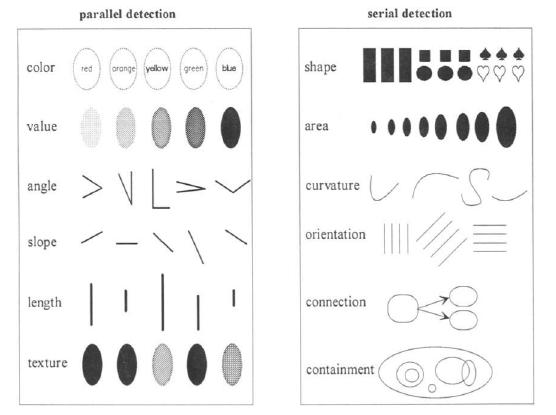
\includegraphics[width=.8\linewidth]{ParallelSerialFeatures}
\caption[Parallel and Serial Feature Detection]{Examples of features detected serially or in parallel (Chapter 6, \protect\citealt{helander1997handbook})}\label{fig:parallelSerialFeatures}
\end{figure}

Feature integration as a result of attention enables the brain to process a figure holistically. This processing is important for the most basic visual processes we take for granted, including object perception. 

\subsubsection{Object Perception} \label{ObjectPerception}
The most basic task of the visual system is to perceive objects in the world around us. This is an inherently difficult task, however, because the retina is a flat, two-dimensional surface responsible for conveying a three-dimensional visual scene. This dimensional reduction means that there are multiple three-dimensional stimuli that can produce the same visual image on the retina. This is known as the inverse projection problem - an infinite number of three-dimensional objects produce the same two-dimensional image. Less relevant to statistical graphics, but still complicating the object perception process, a single object can be viewed from a multitude of angles, in many different situations which may affect the retinal image (lighting, partial obstruction, etc). These problems mean that the brain must utilize many different heuristics to increase the accuracy of the perceived world relative to an ambiguous stimulus. 

The most commonly cited set of heuristics for object perception (and the set most relevant to statistical graphics) are known as the \emph{Gestalt Laws of Perceptual Organization} (\citealt{goldstein}, Chapter 5.2). These laws are related to the idea ``the whole is greater than the sum of the parts'', that is, that the components of a visual stimulus, when combined, create something that is more meaningful than the separate components considered individually. 

\begin{itemize}
\item \textbf{Pragnanz - the law of good figure}. Every stimulus pattern is seen so that the resulting structure is as simple as possible. 
\item \textbf{Proximity}. Things that are close in space appear to be grouped. 
\item \textbf{Similarity}. Similar items appear to be grouped together. The law of similarity is usually subordinate to the law of proximity. 
\item \textbf{Good Continuation}. Points that can be connected to form straight lines or smooth curves seem to belong together, and lines seem to follow the smoothest path. 
\item \textbf{Common Fate}. Things moving in the same direction are part of a single group.
\item \textbf{Familiarity}. Things are more likely to form groups if the groups are familiar. 
\item \textbf{Common Region}. Things that are in the same region (container) appear to be grouped together
\item \textbf{Uniform Connectedness}. A connected region of objects is perceived as a single unit.
\item \textbf{Synchrony}. Events occurring at the same time will be perceived as belonging together.
\end{itemize}

\subsubsection{Visual Memory}
We have discussed how visual stimuli are perceived and how objects are recognized; we now must examine how visual stimuli are encoded into memory. Most researchers believe that visual perceptions are encoded in an analog fashion, so that the memory of an image is closely related to the perception of that same image \citep{cognition}. Other theories suggest that visual perceptions are encoded semantically, that is, the description of a visual scene would be encoded, rather than a mental ``image" of that scene. Both theories are likely at least partially correct, but the analog encoding of visual images is more relevant to statistical graphics because the accuracty of the stored image has the potential to affect recall of the contents of that image (and thus what people remember about a particular graphic). Experimental evidence for analog encoding includes the mental rotation task, where participants must determine whether or not a figure is a rotation of a target figure, as shown in Figure \ref{fig:mentalRotation}. \citet{shepard1988mental} showed that reaction time was proportional to the angle of rotation of the stimuli, which suggests that participants were mentally rotating the figure as they would rotate a three-dimensional figure in space. 


\begin{figure}[h]\centering
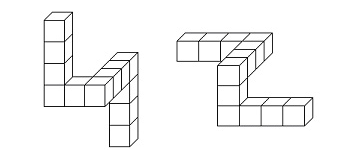
\includegraphics[width=.7\textwidth]{RotationTask}
\caption[Rotation Task]{Rotation task \protect\citep{shepard1988mental}. Are the two images the same?}\label{fig:mentalRotation}
\end{figure}

In addition, \citet{kosslyn1978visual} showed that mental representation of distances in a figure are accurate and that the time to encode those distances is proportional to the distances in the actual figure. These studies suggest that the memory of an image (statistical graphic or otherwise) is a reasonably accurate facsimile of the original image (though this is of course likely to be moderated by attention and recall ability). 

Another facet of visual memory that will be important to understanding perception and memory of statistical graphics is that the ``gist" of an image is stored along with the image. In these cases, recall ability is more consistent with the semantic encoding of images; that is, when shown an ambiguous figure (such as Figure \ref{fig:ambiguousrabbit}) and asked to describe it initially, participants could not give an alternate interpretation of the figure after the experiment was complete. In the case of  Figure \ref{fig:ambiguousrabbit}, participants who initially said the figure was a duck could not describe the figure as a rabbit later, even though the image is consistent with either interpretation. This suggests that in some cases, verbal encoding of a figure (i.e. describing it as a duck) disrupts the mental representation of the picture. This is common in other types of memories as well: when the gist of a passage is stored, the actual content of the passage is no longer accessible. In other words, we would expect that if someone had to interpret a graph, they would remember the interpretation much more strongly than the actual graph, even if that interpretation was incorrect or incomplete. 

\begin{figure}[h]\centering
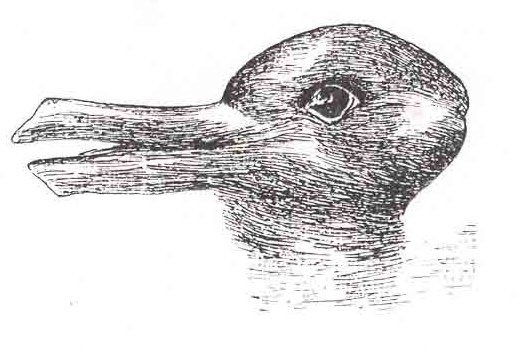
\includegraphics[width=.4\textwidth]{DuckRabbitIllusion}
\caption[Ambiguous Images]{An ambiguous image that could be either a rabbit or a duck. When participants were asked to identify the image initially, they could not provide an alternate interpretation of the figure later.}\label{fig:ambiguousrabbit}
\end{figure}

The ``software" of the visual system is of course more complex than the few programs listed here, but understanding attention, object perception concepts, and how images are stored for later retrieval in the brain will make designing statistical graphics for the visual system easier and will also help with evaluating graphics based on the capabilities of the human visual system. 

\subsection{Bugs and Peculiarities of the Visual System}
We have discussed the neural ``hardware" of the visual system and some of the higher-level processing that contributes to our ability to create and understand meaning in the world around us. Occasionally, our highly tuned perceptual system fails in unusual ways due to the heuristics and algorithms that were optimized for operation in a three-dimensional world where the main tasks were hunting, gathering, and avoiding predators. We will examine three interesting results of this tuning that are important to the design of statistical graphics as we transition from the psychophysics and cognitive psychology literature to statistics and human-computer interaction literature. 

\subsubsection{Logarithmic perception} One of the earliest psychophysics researchers, Ernst Weber, discovered that the difference threshold, the smallest detectable difference between two sensory stimuli, increased proportionately with the magnitude of the stimulus. This statement, known now as Weber's Law, holds true for a large range of intensities of a number of senses. Numerically, Weber's Law is stated as 
\begin{equation}\label{weberlaw}
\frac{\triangle S}{S} = K
\end{equation}
where $K$ is a constant called the Weber fraction, $S$ is the value of the standard stimulus, and $\triangle S$ is the difference between the standard stimulus and the test stimulus. So if a participant is given a 100-g weight and a 102-g weight and can just barely tell the difference between the two, then $K=0.02$ and we would assume that the the difference between a 200-g weight and a 204-g weight would be just barely detectable as well (Chapter 1, \citealt{goldstein}). While this example concerns the ability to distinguish weight, the same law holds for the ability to distinguish sounds of different intensities as well as intensity of colors. The tendency of the brain to perceive stimuli in a logarithmic fashion is true across many perceptual domains. In fact, when kindergarden children are asked to place numbers 1-10 along a number line, they place 3 in about the middle, just as one would expect from a logarithmic perspective. This ability disappears with mathematical education, but persists in those who are not given a formal education in mathematics, indicating that our brains are naturally wired to perceive numbers logarithmically as well \citep{varshney2013we}. In some sensory domains, even the scales used to measure stimuli such as sound intensity, earthquake intensity, and frequency along the electromatic spectrum are logarithmic. Information theory suggests that logarithmic scaling provides optimal compression of information to minimize relative errors in perception while accounting for limits in our neural bandwidth. \citet{sun2012framework} showed that a bayesian model for perception would result in a model that mimics the logarithmic relationship in Weber's Law. This suggests that the logarithmic nature of human perception is a result of an heuristic that increases processing power by reducing the neural bandwidth necessary to process information through quantization of continuous information and compression of discrete information. 

From a statistical graphics point of view, then, log-transformed scales should be used instead of linear scales for continuous color scales, as this provides more information discrimination ability and mimics natural human perceptual tendencies. 

\todo[inline]{Expand this? Move? }

\subsubsection{Colorblindness and color perception}
Another common ``bug" in the visual system are mutations that change (or remove entirely) the cones in the retina. Such mutations are commonly termed ``colorblindness" and encompass many different types of mutations, shifts and deletions that affect color perception in the visual system. These mutations affect up to 5\% of the population, and are generally more common in males than they are in females, as two of the three genes producing cones are found on the X chromosome. Evolutionarily, these mutations are maladaptive for gathering plants, but may be adaptive for seeing camoflauged objects \citep{morgan1992dichromats}. In statistical graphics, however, these mutations often disrupt perception of standard color schemes used in maps, heatmaps, and divergent color scalings. Figure \ref{fig:USflag} shows the us flag as seen by those with different types of color-blindness; the red and blue hues look radically different to those with different mutations. 

\begin{figure}[h]\centering
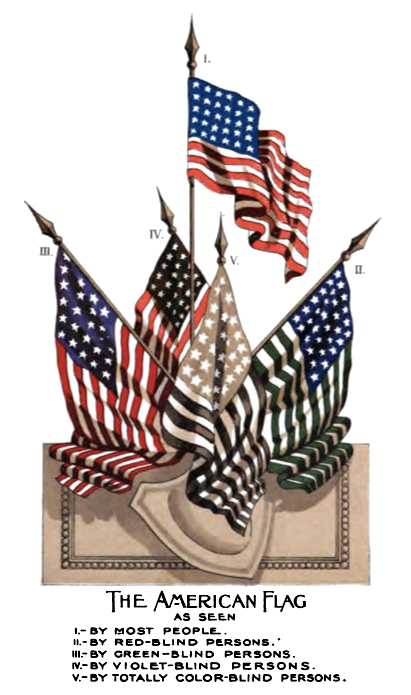
\includegraphics[width=.3\textwidth]{USflagColorBlind}
\caption{An 1895 illustration of the US flag as seen by those with different types of colorblindness.}\label{fig:USflag}
\end{figure}



\subsubsection{Optical Illusions}


\section{Statistical Graphics}
\subsection{Low-level perception of graphics}\label{LowLevelGraphics}
Healey's preattentive feature integration stuff
\subsection{Higher-level graphical perception}\label{HighLevelGraphics}
\begin{itemize}
\item Cleveland \& McGill
\item Heuristic guidelines i.e. Kosslyn and Tufte
\item Grammar of graphics allows us to test graphics which display the same information in different ways for comparable accuracy
\end{itemize}
Emphasize the low-level stuff vs. the higher-level stuff that focuses on preattentive information (i.e. not what we care about) and the gap in the middle where graphics are tested in more practical scenarios.

\subsection{Optical illusions and statistical graphics}
three-dimensional context, other ways to trigger optical illusions with graphics. Importance of being aware of the heuristics the brain uses so that problematic graphics can be avoided. 

\subsection{Interactive graphics?} 
Not sure if this should be a subsection, but graphics that respond to human interaction violate the two-dimensional graphic paradigm somewhat, which means there are a whole 'nother set of issues to consider... motion illusions, grouping, etc.

\section{Testing Statistical Graphics}
Methodology for testing graphical perception in humans. Talk about masking, the power of suggestion, habituation, etc. as well as paradigms - search and find, response time, numerical judgments, signal detection, eye tracking. 
\begin{itemize}
  \item Tukey
  \item Cleveland \& McGill
  \item Lineups
\end{itemize}

\end{document}
